\documentclass[oneside]{ZJUthesis}
% 该文档中首字符为“%”的均为注释行,不会在论文中出现

% 论文默认为单面模式,需单面模式请将第一行换为如下所示:
% \documentclass[twoside]{ZJUthesis}

% 取消目录中链接的颜色,方便打印
% 如需颜色,请将“false”改为“true”
\hypersetup{colorlinks=true}

% 这里几行代码使得目录中的“第几章” 和后面的章节名称不致发生重叠
\makeatletter
\renewcommand{\numberline}[1]{%
\settowidth\@tempdimb{#1\hspace{0.5em}}%
\ifdim\@tempdima<\@tempdimb%
  \@tempdima=\@tempdimb%
\fi%
\hb@xt@\@tempdima{\@cftbsnum #1\@cftasnum\hfil}\@cftasnumb}
\makeatother


\begin{document}
%%%%%%%%%%%%%%%%%%%%%%%%%%%%%
%% 正文字体设定
%%%%%%%%%%%%%%%%%%%%%%%%%%%%%
\songti

%%%%%%%%%%%%%%%%%%%%%%%%%%%%%
%% 论文封面部分
%%%%%%%%%%%%%%%%%%%%%%%%%%%%%
% 中文封面内容

% 中图分类号
\classification{TM863}

% 单位代码
\serialnumber{10335}

% 密级,如需密级则将其前“%”去掉
%\SecretLevel{绝密}

% 学号
\PersonalID{11011010}

\title{基于成本的钉耙强度与应用}
% 如果标题一行写不下,就写成两行,在下面的命令里写第二行,不需要两行则注释掉
\titletl{——东方视角分析}

%英文题目
\Etitle{Cost Based Rake Strength}
% 如果一行写不下,同中文题目设定,一行写不下则写两行,不需要就注释掉
\Etitletl{and Application:}
\Etitletll{An Oriental View}

% 作者
\author{猪八戒}
\Eauthor{Bajie Zhu}

\degree{硕士}
\Edegree{Master of Engineering}

% 导师
\supervisor{唐三藏法师}
\Esupervisor{Master Sanzang Tang}

% 合作导师,如果有的话,去掉注释,
% \cpsupervisor{张三丰真人}
% \Ecpsupervisor{Truman Sanfeng Zhang}

% 专业名称
\major{祭坛管理}
\Emajor{Altar Management}

% 研究方向
\researchdm{法器工程}
\Eresearchdm{Ritual Instrument Engineering}

% 所属学院
\institute{大雷音寺管理研究院}
\Einstitute{Management Institute of Great Thunder Monastery}

%论文提交日期
\submitdate{二〇一三年一月十日}
\Esubmitdate{2013-1-10}

% 答辨日期
%\defenddate{2011年11月1日}

% 生成封面
\makeCoverPage

% 生成英文封面
\makeECoverPage

%%%%%%%%%%%%%%%%%%%%%%%%%%%%%%
%% 原创声明与版权协议页
%%%%%%%%%%%%%%%%%%%%%%%%%%%%%%

% 生成原创声明与版权协议页
\makeOSandCPRTpage


%%%%%%%%%%%%%%%%%%%%%%%%%%%%%%
%% 论文部分开始
%%%%%%%%%%%%%%%%%%%%%%%%%%%%%%
\ZJUfrontmatter

%%%%%%%%%%%%%%%%%%%%%%%%%%%%%%
%% 摘要
%%%%%%%%%%%%%%%%%%%%%%%%%%%%%%
\begin{abstract}
这是一篇有关法器钉耙的研究。以往法器研究都是从西方视角出发,没有考虑东方文化背景的影响。本研究结合钉耙在农业中的广泛应用,对钉耙的作用进行开创性研究。

扯几句,再扯几句。

\keywords{钉耙,成本,法器,\LaTeX}
\end{abstract}


%%%%%%%%%%%%%%%%%%%%%%%%%%%%%%
%% 英文摘要
%%%%%%%%%%%%%%%%%%%%%%%%%%%%%%
\begin{englishabstract}
Rake is good. My rake has nine prongs. Rake can be used in farm. Blur, blur, blur...

\englishkeywords{rake, cost, \XeTeX}
\end{englishabstract}


%%%%%%%%%%%%%%%%%%%%%%%%%%%%%%
%% 目录页
%%%%%%%%%%%%%%%%%%%%%%%%%%%%%%
\ZJUcontents

%%%%%%%%%%%%%%%%%%%%%%%%%%%%%%
%% 插图列表
%%%%%%%%%%%%%%%%%%%%%%%%%%%%%%
\ZJUListofFigures

%%%%%%%%%%%%%%%%%%%%%%%%%%%%%%
%% 表格列表
%%%%%%%%%%%%%%%%%%%%%%%%%%%%%%
\ZJUListofTables


%%%%%%%%%%%%%%%%%%%%%%%%%%%%%%
%% 正文内容部分开始
%%%%%%%%%%%%%%%%%%%%%%%%%%%%%%
\ZJUmainmatter

\chapter{绪论}

这是的示例文档。格式样列很大一部分是直接从薛瑞尼的 {《清华大学学位论文 \LaTeX 模板》,\url{http://thuthesis.sourceforge.net/}} 示例文档中拿来的。

\section{字体示例}

九齿钉耙学名{\kaishu 上宝沁晶耙},是俺的武器。九齿钉耙并非普通的农具,而是由太上老君\footnote{太上老君,三清之第三位。又称“道德天尊”、“混元老君”、“降生天尊”、“太清大帝”等。}用神冰铁亲自锤炼,借五方五帝、六丁六甲之力锻造而成,有诗为证:

\vspace{-5mm}

\begin{tabbing}
\hspace{20mm} \= \hspace{20mm} \= \hspace{80mm} \kill\\
 \> 字体      \>  \hspace{26mm} 示例 \\
 \> fangsong \> \fangsong 老君自己动钤锤,荧惑亲身添炭屑。 \\
 \>          \> \fangsong 五方五帝用心机,六丁六甲费周折。 \\
 \>          \> \fangsong 造成九齿玉垂牙,铸就双环金坠叶。 \\
 \> heiti    \> \heiti 身妆六曜排五星,体按四时依八节。 \\
 \>          \> \heiti 短长上下定乾坤,左右阴阳分日月。 \\
 \>          \> \heiti 六爻神将按天条,八卦星辰依斗列。 \\
 \> kaishu    \> \kaishu 名为上宝沁金钯,进与玉皇镇丹阙。 \\
 \>          \> \kaishu 因我修成大罗仙,为吾养就长生客。 \\
 \>          \> \kaishu 敕封元帅号天蓬,钦赐钉钯为御节。 \\
 \> lishu    \> \lishu 举起烈焰并毫光,落下猛风飘瑞雪。 \\
 \>          \> \lishu 天曹神将尽皆惊,地府阎罗心胆怯。 \\
 \>          \> \lishu 人间那有这般兵,世上更无此等铁。 \\
 \> songti   \> \songti 随身变化可心怀,任意翻腾依口诀。 \\
 \>          \> \songti 相携数载未曾离,伴我几年无日别。 \\
 \>          \> \songti 日食三餐并不丢,夜眠一宿浑无撇。 \\
 \> youyuan    \> \youyuan 也曾佩去赴蟠桃,也曾带他朝帝阙。 \\
 \>          \> \youyuan 皆因仗酒却行凶,只为倚强便撒泼。 \\
 \>          \> \youyuan 上天贬我降凡尘,下世尽我作罪孽。 \\
 \> default  \> 石洞心邪曾吃人,高庄情喜婚姻结。 \\
 \>          \> 这钯下海掀翻龙鼍窝,上山抓碎虎狼穴。 \\
 \>          \> 诸般兵刃且休题,惟有吾当钯最切。 \\
 \>          \> 相持取胜有何难,赌斗求功不用说。 \\
 \>          \> 何怕你铜头铁脑一身钢,钯到魂消神气泄!
\end{tabbing}

\section{各种示例}

没有规定英文字体,将中、英文统一设置为仿宋。

当存在连续多个表格、图片时,\LaTeX 的排版效果不佳,所以这里不时插播些王勃的《腾王阁序》,有空的话也看两眼。

《腾王阁序》第一段:豫章故郡,洪都新府。星分翼轸,地接衡庐。襟三江而带五湖,控蛮荆而引瓯越。物华天宝,龙光射牛斗之墟;人杰地灵,徐孺下陈蕃之榻。雄州雾列,俊采星驰。台隍枕夷夏之交,宾主尽东南之美。都督阎公之雅望,棨戟遥临;宇文新州之懿范,襜帷暂驻。十旬休假,胜友如云;千里逢迎,高朋满座。腾蛟起凤,孟学士之词宗;紫电青霜,王将军之武库。家君作宰,路出名区,童子何知,躬逢胜饯。

《腾王阁序》第二段:时维九月,序属三秋。潦水尽而寒潭清,烟光凝而暮山紫。俨骖騑于上路,访风景于崇阿。临帝子之长洲,得天人之旧馆。层台耸翠,上出重霄;飞阁翔丹,下临无地。鹤汀凫渚,穷岛屿之萦回;桂殿兰宫,即冈峦之体势。披绣闼,俯雕甍:山原旷其盈视,川泽纡其骇瞩。闾阎扑地,钟鸣鼎食之家;舸舰迷津,青雀黄龙之轴。云销雨霁,彩彻区明。落霞与孤鹜齐飞,秋水共长天一色。渔舟唱晚,响穷彭蠡之滨;雁阵惊寒,声断衡阳之浦。

\subsection{图片示例}

附上照片一张,来源 Wikipedia。

\begin{figure}[htbp]
  \centering
  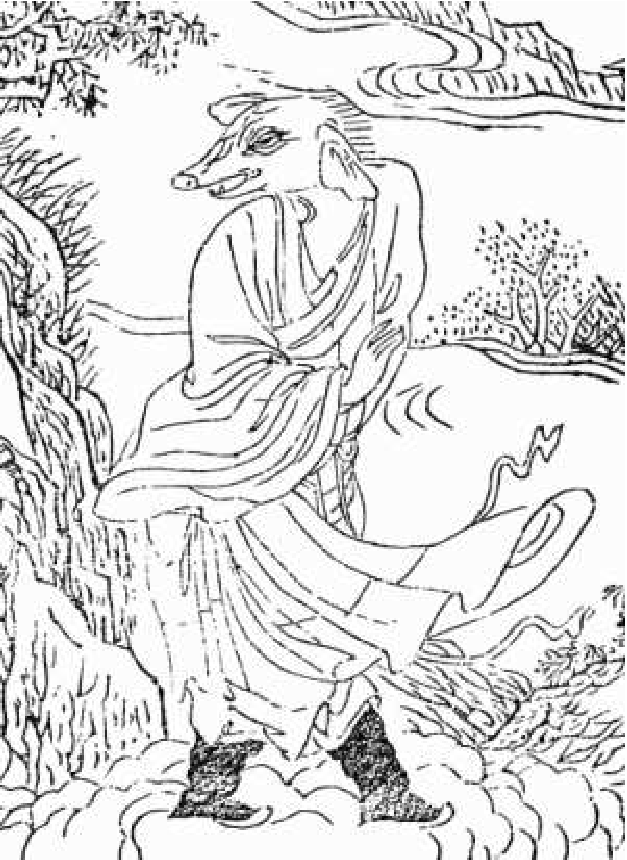
\includegraphics[scale=0.8]{./images/zhubajie.pdf}
  \caption{玉照,玉做的照片,通常会令人联想到浴照。}
  \label{fig:example}
\end{figure}

我来插两张并排的图像,其实\LaTeX 支持jpg, png, 以及eps格式的图片,图\ref{fig:tangseng}是我的师傅,帅吧!

\begin{figure}[htbp]
\centering
\subfloat[师傅]{
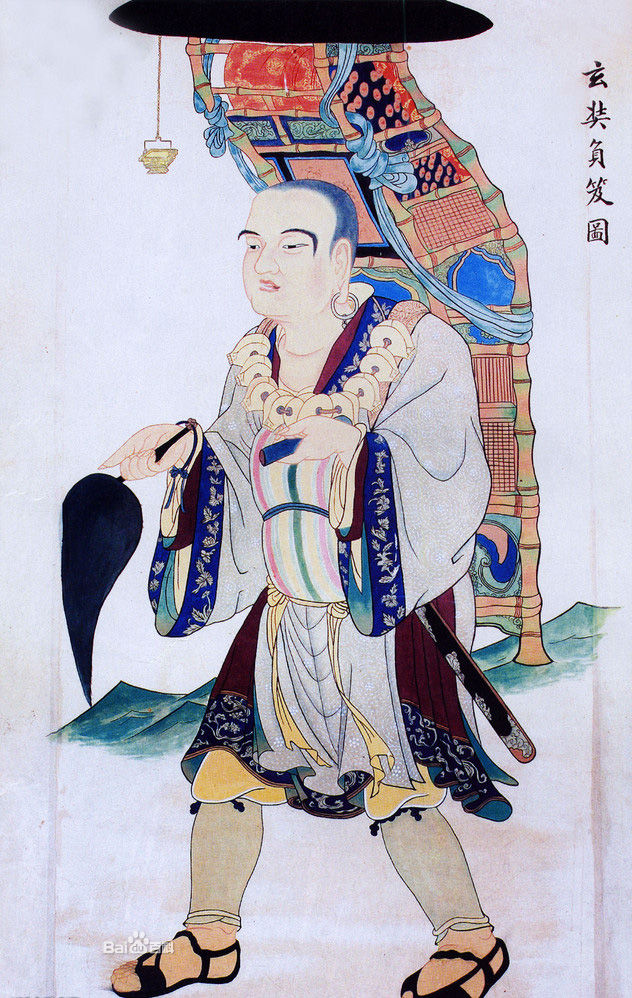
\includegraphics[width=6cm]{./images/tangseng.jpg}
\label{fig:tangseng}
}
\hspace{60pt}
\subfloat[大师兄]{
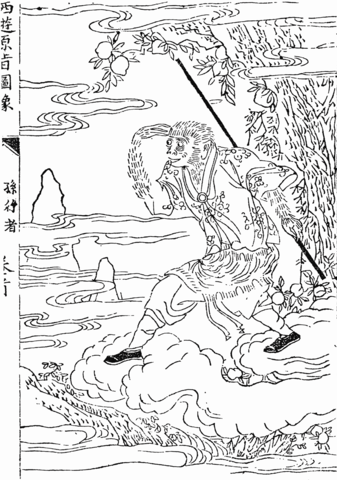
\includegraphics[width=6cm]{./images/sunwukong.png}
\label{fig:sunwukong}
}
\caption{你挑着担,我写代码...}
\end{figure}

\subsection{表格示例}

\LaTeX 中的表格不是很好搞,看起来很不直观,不过我们一般不会用太高端的表格,更多关于表格的请看\texttt{Helin Gai}的\textsf{\LaTeX Manual}\cite{gaiart}以及
\texttt{Alpha Huang}的\textsf{lnotes}\cite{lnotes}

先看一个简单表格 \ref{tab:simple-table}:

\begin{table}[htb]
  \centering
  \caption{模板中的表格宏包}
  \label{tab:simple-table}
    \begin{tabular}{ll}
      \toprule
      \multicolumn{1}{m{20mm}}{\heiti\centering 宏包} & \multicolumn{1}{m{80mm}}{\heiti\centering 描述} \\
      \midrule
      longtable & 绘制跨页的表格。 \\
      booktabs & 三线表中的那三条线的命令来自这里。\\
      caption2 & 用于设置标题很方便,已经 obsolated,不过 \TeX Live 中还有。\\
      multirow & 跨行的单元格用这个宏包。\\
      dcolumn  & 想让表格小数点对齐吗?用这个宏包吧。\\
      \rowcolor[gray]{.9} colortbl & 表格上色。自己看着爽而已,打印出来都是黑白的。 \\
      threeparttable & 用来给表格添加脚注啥的很方便。 \\
      array & 忘了用来做什么了,但似乎很重要。 \\
      \bottomrule
    \end{tabular}
\end{table}


\subsection{公式示例}

我公式用非常少,所以公式的情况并不了解,这部分示例也完全照搬 。如果有什么问题或要求,可以贴到 88 \TeX 版。

贝叶斯公式如式 (\ref{equ:chap1:bayes}),其中 $p(y|\mathbf{x})$ 为后验;$p(\mathbf{x})$ 为先验;分母 $p(\mathbf{x})$ 为归一化因子。

\begin{equation}
\label{equ:chap1:bayes}
p(y|\mathbf{x}) = \frac{p(\mathbf{x},y)}{p(\mathbf{x})}=
\frac{p(\mathbf{x}|y)p(y)}{p(\mathbf{x})} 
\end{equation}

论文里面公式越多,\TeX 就越 happy。再看一个 \textsf{amsmath} 的例子:

\newcommand{\envert}[1]{\left\lvert#1\right\rvert} 

\begin{equation}\label{detK2}
\det\mathbf{K}(t=1,t_1,\dots,t_n)=\sum_{I\in\mathbf{n}}(-1)^{\envert{I}}
\prod_{i\in I}t_i\prod_{j\in I}(D_j+\lambda_jt_j)\det\mathbf{A}
^{(\lambda)}(\overline{I}|\overline{I})=0.
\end{equation} 

大家在写公式的时候一定要好好看 \textsf{amsmath} 的文档,并参考模板中的用法:

\begin{multline*}\tag{[b]} % 这个出现在索引中的
\int_a^b\biggl\{\int_a^b[f(x)^2g(y)^2+f(y)^2g(x)^2]
 -2f(x)g(x)f(y)g(y)\,dx\biggr\}\,dy \\
 =\int_a^b\biggl\{g(y)^2\int_a^bf^2+f(y)^2
  \int_a^b g^2-2f(y)g(y)\int_a^b fg\biggr\}\,dy
\end{multline*}

其实还可以看看这个多级规划:

\begin{equation}\label{bilevel}
\left\{\begin{array}{l}
\max\limits_{{\mbox{\footnotesize\boldmath $x$}}} F(x,y_1^*,y_2^*,\cdots,y_m^*)\\[0.2cm]
\mbox{subject to:}\\[0.1cm]
\qquad G(x)\le 0\\[0.1cm]
\qquad(y_1^*,y_2^*,\cdots,y_m^*)\mbox{ solves problems }(i=1,2,\cdots,m)\\[0.1cm]
\qquad\left\{\begin{array}{l}
    \max\limits_{{\mbox{\footnotesize\boldmath $y_i$}}}f_i(x,y_1,y_2,\cdots,y_m)\\[0.2cm]
    \mbox{subject to:}\\[0.1cm]
    \qquad g_i(x,y_1,y_2,\cdots,y_m)\le 0.
    \end{array}\right.
\end{array}\right.
\end{equation}

\subsection{定理示例}

THUThesis定义了很多定理格式,THUThesis下面都是从来的例子。我自己只用到了“假设”,对于公式、证明之类的格式完全无知,你如有其他需要可以在 88 \TeX 版上提出来,我再添加。

\begin{hypo}
待月西厢下,迎风户半开;隔墙花影动,疑是玉人来。
\begin{eqnarray}
  \label{eq:eqnxmp}
  c & = & a^2 - b^2\\
    & = & (a+b)(a-b)
\end{eqnarray}
\end{hypo}

\begin{defin}
子曰:「道千乘之国,敬事而信,节用而爱人,使民以时。」
\end{defin}

\begin{theo}
犯我强汉者,虽远必诛。\hfill —— 陈汤(汉)
\end{theo}

\begin{pro}
天不言自高,水不言自流。
\begin{gather*}
\begin{split} 
\varphi(x,z)
&=z-\gamma_{10}x-\gamma_{mn}x^mz^n\\
&=z-Mr^{-1}x-Mr^{-(m+n)}x^mz^n
\end{split}\\[6pt]
\begin{align} \zeta^0&=(\xi^0)^2,\\
\zeta^1 &=\xi^0\xi^1,\\
\zeta^2 &=(\xi^1)^2,
\end{align}
\end{gather*}
\end{pro}

\subsection{算法示例}

大家有时候还需要写一些算法的伪代码,不用蛋疼,模板里面已经有支持了,看看算法\ref{alg:put-into-refri},具体的实用还需要参考CTAN上的关于{\textsf{algorithmicx}}宏包的文档,包括自定义关键字等等。

\begin{algorithm}
\caption{把猪八戒放进冰箱}
\label{alg:put-into-refri}
\begin{algorithmic}[1]
\Require N头动物,不知道是不是猪八戒  \Comment{我是注释} 
\Ensure 你造吗,这个程序木有输出,想怎样?
\State 先热热身:)
\For{$i=1,\dots ,N$} \Comment{我是个For循环}
\If {是猪八戒}
	\State 打开冰箱门,把第$i$个放进冰箱,关上冰箱门
\Else 
	\State 下一个
\EndIf
\EndFor
\end{algorithmic}
\end{algorithm}

\subsection{参考文献}

参考文献建议使用 BiB\TeX 。

参考文献的例子:书籍文献\cite{tex,companion};杂志文章,单独的\cite{article1},并列的\cite{article2,article3},合并的\cite{article1,article2,article3};硕士论文\cite{master},俺的旧文一篇;博士论文\cite{doctor},沙师弟的大作;论文集或 Handbook\cite{collection},会议论文集\cite{proceeding},会议论文\cite{conference};带页码脚标的\cite[123]{tex}。




\chapter{第二章}

这是第二章,目的是占个位置。你知道《浙大同学爱占坐》这首歌吗?


\ZJUbackmatter
%%%%%%%%%%%%%%%%%%%%%%%%%%%%%%
%% 参考文献
%%%%%%%%%%%%%%%%%%%%%%%%%%%%%%
\ZJUthesisbib{thesisbib}

%%%%%%%%%%%%%%%%%%%%%%%%%%%%%%
%% 发表论文目录
%%%%%%%%%%%%%%%%%%%%%%%%%%%%%%
\begin{publications}
\begin{itemize}
\item 猪八戒,猪悟能,天蓬元帅,等. 论流体食物的持久保存 [D]. 硕士学位论文. 北京: 广寒宫大学, 2005
\end{itemize}

\end{publications}


%%%%%%%%%%%%%%%%%%%%%%%%%%%%%%
%% 致谢页
%%%%%%%%%%%%%%%%%%%%%%%%%%%%%%
\begin{thanks}
感谢导师唐三藏的温柔和慈爱,不计时间给予俺无微不至地教诲,让俺在如雨般的唾沫星下滋润成长。

感谢师兄孙悟空的肢体教育,让俺成功减肥,俺和俺身上的每一块青紫都会记住你的。

感谢师弟沙悟净的任劳任怨,得失无争。

感谢高小姐的一片真情,可叹俺已遁入空门、修成正果。当年你在情人坡娇怨俺没貌没地位,现在俺终于位列仙班,可却注定要永远分离,缘何俺们总是“错位”……

\begin{flushright}
{\lishu{
  \large{猪悟能}\hspace{0.5in}

  \large{2013年1月于大雷音寺}\hspace{0.18in}
}}

\end{flushright}

\end{thanks}



\end{document}
